%%%%%%%%%%%%%%%%%%%%%%
% INTRODUCTION TO THE COALESCENT
%%%%%%%%%%%%%%%%%%%%%%

\begin{frame}
\frametitle{The coalescent}

Data: a \alert{small genetic sample} from a \alert{large background population}.

\smallskip 
\alert{The coalescent }
\begin{itemize}
\item is a model of the ancestral relationships of a sample of individuals taken from a larger population.
\smallskip
\item describes a probability distribution on ancestral genealogies (trees) given a population history, $N(t)$. 
  \begin{itemize}
	\item Therefore the coalescent can convert information from ancestral genealogies into information about population history and vice versa.
  \end{itemize}
\smallskip
\item a model of ancestral genealogies, not sequences, and its simplest form assumes neutral evolution.
\smallskip
\item can be thought of as a prior on the tree, in a Bayesian setting.
\end{itemize}

\end{frame}

\begin{frame}
\frametitle{The coalescence of two ancestral lineages}

\begin{columns}

\column{.64\textwidth}

\begin{itemize}
\item First, consider two random members from a population of fixed size $N$. 

\item By perfect mixing, the probability they share a \emph{concestor} in the previous generation is $1/N$. 

\item The probability the concestor is $t$ generations back is 

\begin{equation*}
Pr\{t\} = \frac{1}{N}(1-\frac{1}{N})^{t-1}. 
\end{equation*}

\item It follows that $g=t-1$, has a geometric distribution with a success rate of $\lambda =
1/N$, and so has mean $N$ and variance of $N^3/(N-1)$.
\end{itemize}

\column{.36\textwidth}
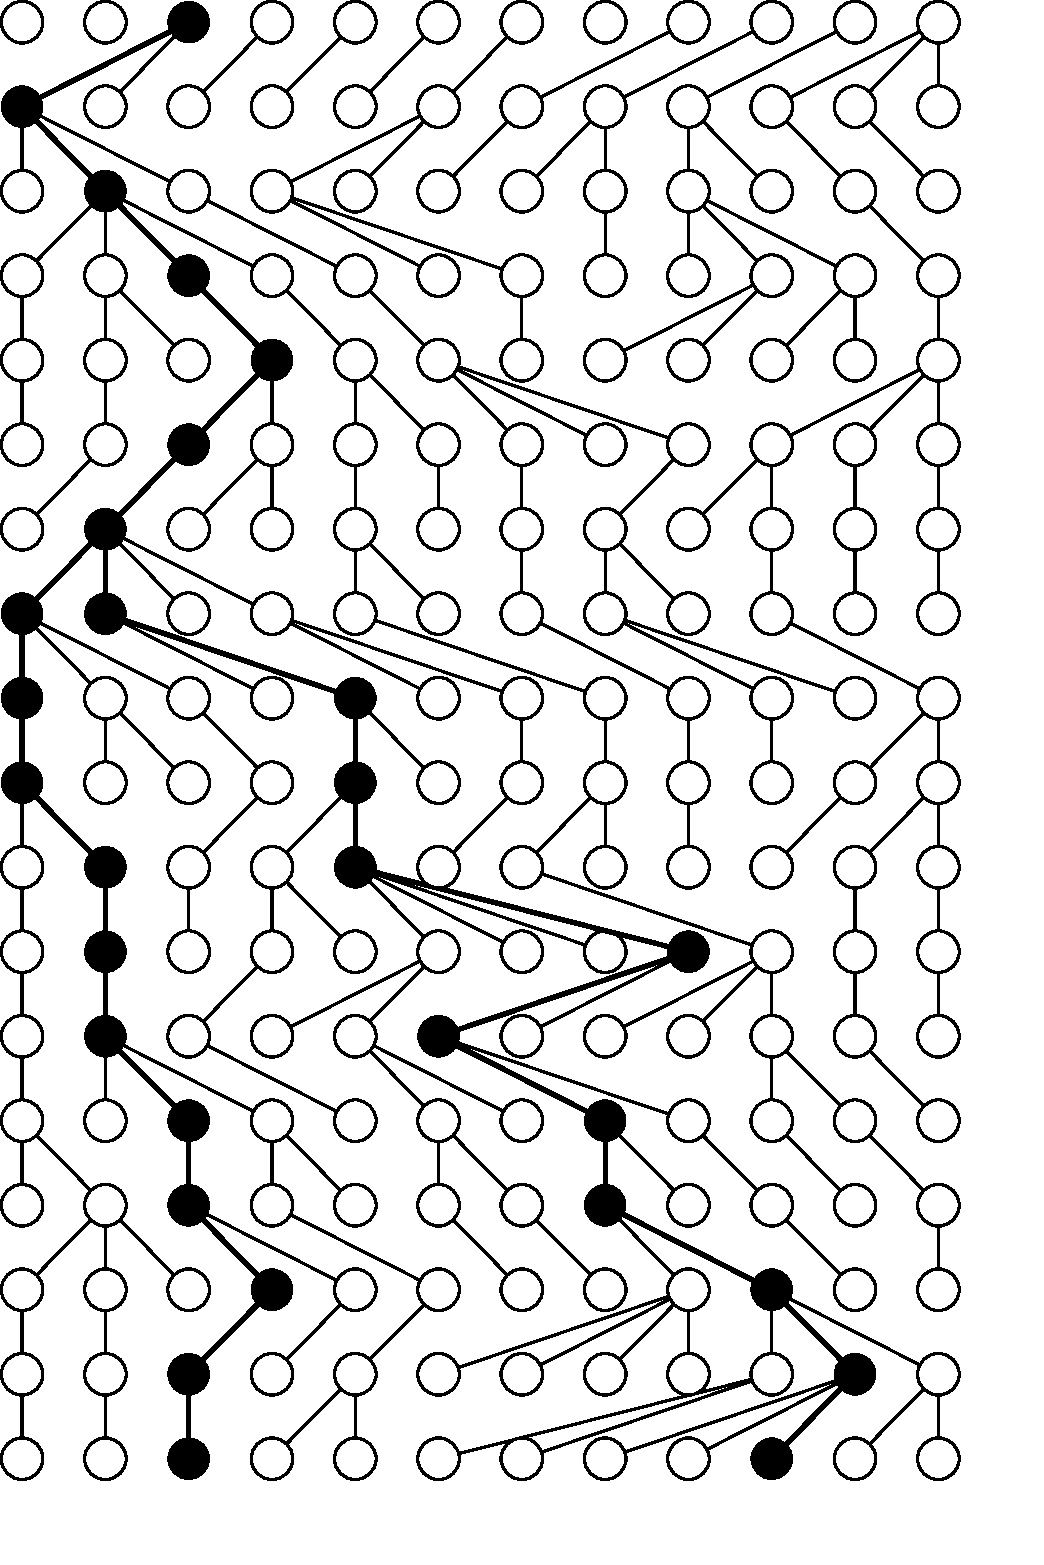
\includegraphics[scale=0.25]{../images/wfCoalescent2}

\end{columns}

\end{frame}

\begin{frame}
\frametitle{The coalescence of $k$ lineages}

\begin{columns}

\column{.64\textwidth}

With $k$ lineages the time to the first coalescence is derived in the same way,
only now there are $\binom{k}{2}$ possible pairs that may coalesce, resulting in
a success rate of $\lambda = \binom{k}{2}/N$ and mean time to first coalescence ($t_k$) of

\begin{equation*}
E[t_k] = \frac{N}{\binom{k}{2}}.
\end{equation*}

This implicitly assumes that $N$ is much larger than $O(k^2)$, so that the probability
of two coalescent events in the same generation is small.


\column{.36\textwidth}
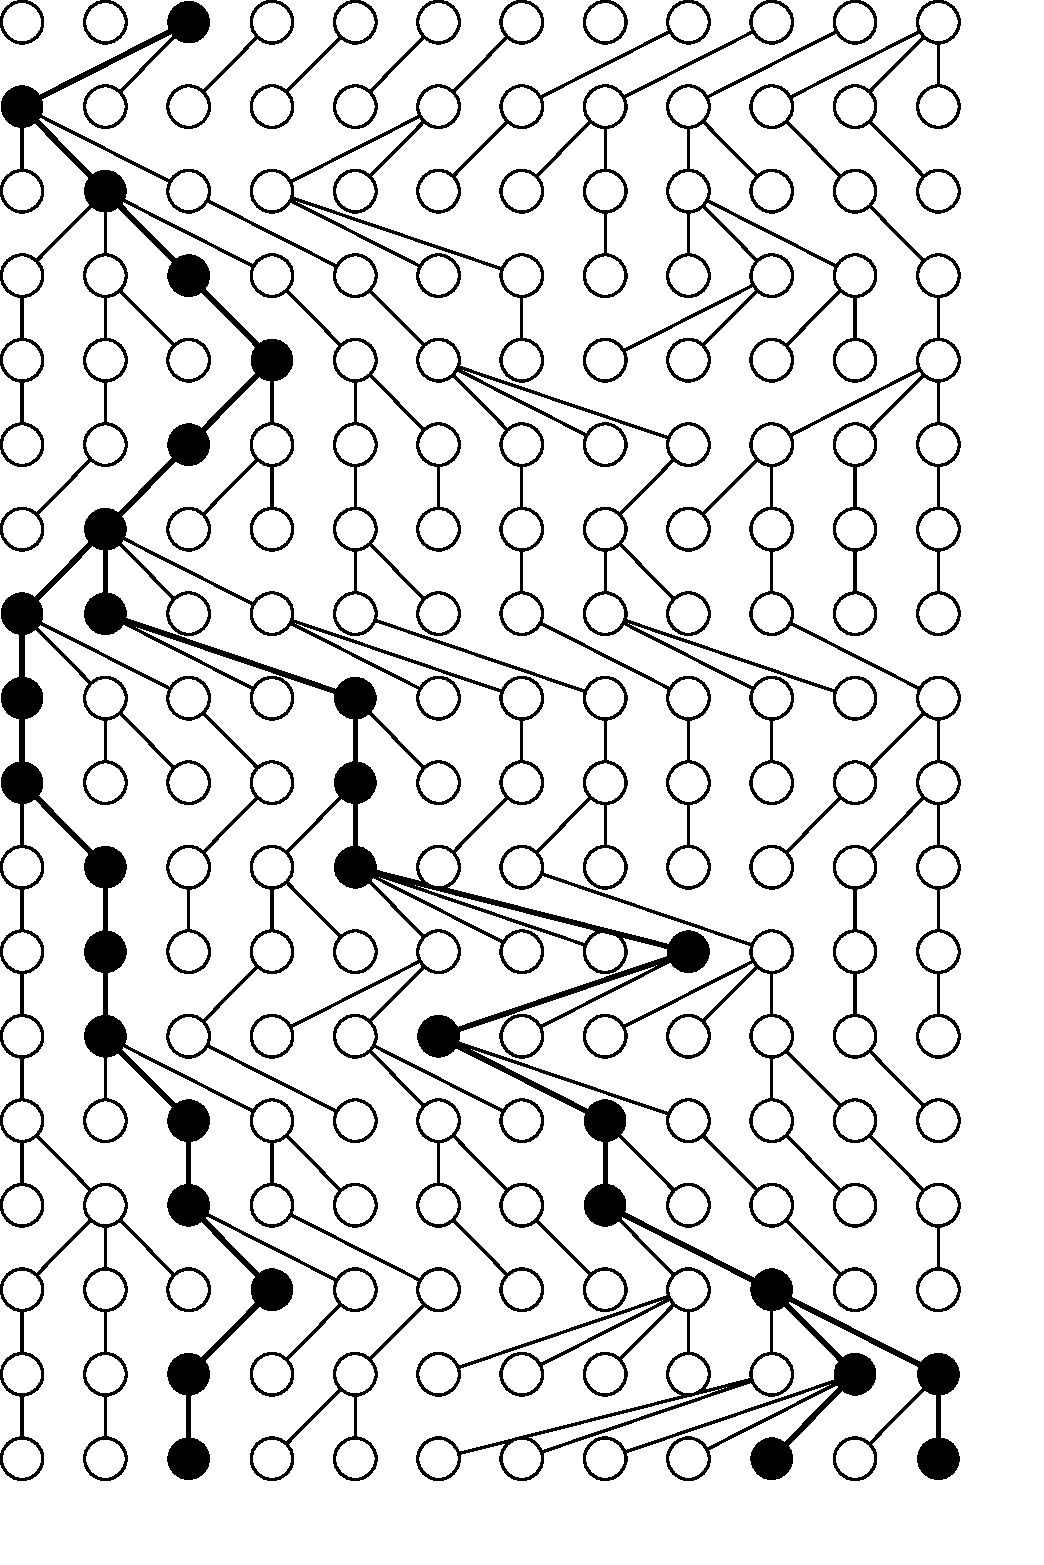
\includegraphics[scale=0.25]{../images/wfCoalescent3}

\end{columns}

\end{frame}


%\begin{frame}
%\frametitle{Some classical coalescent results}

%An interesting consequence is that the average number of generations required for all $k$ lineages to
%coalesce into one is 

%\begin{equation}
%E[t_{root}] = \sum_{i=2}^k \frac{N}{\binom{i}{2}} = 2N(1-\frac{1}{k}), 
%\end{equation}

%which approaches $2N$ as $k$ increases.

%\end{frame}


\begin{frame}
\frametitle{The coalescent is a \emph{diffusion approximation}}

Kingman (1982) showed that as $N$ grows the coalescent process converges to a
continuous-time Markov chain.

\medskip
\begin{columns}[t]

\column{0.5\textwidth}

$\lambda = \binom{k}{2}/N$ is the rate of coalescence, i.e. the probability of coalescing a pair from $k$ lineages on a short time
interval $\Delta t$ is $O({\lambda\Delta t})$. Unsurprisingly the solution turns
out to be the exponential distribution:

\column{0.5\textwidth}

%\center{
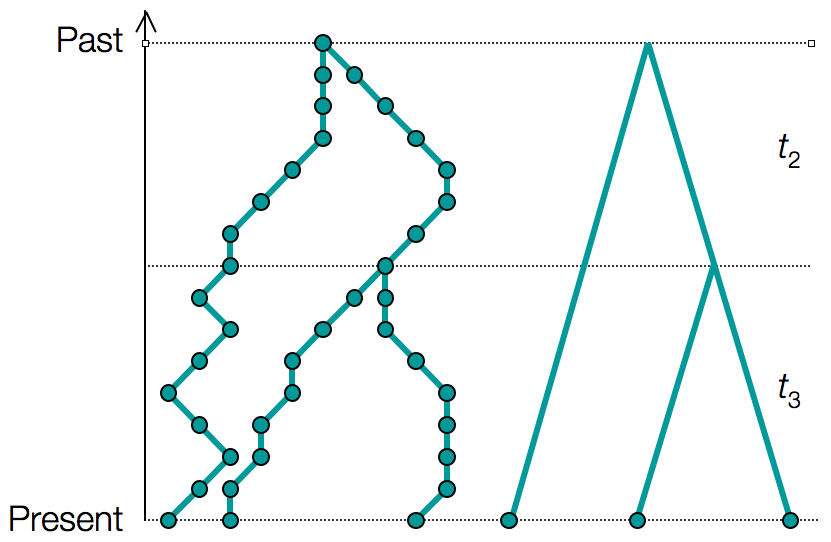
\includegraphics[scale=0.18]{../images/wrightFisherToTree}

%{\small{discrete versus continuous}}
%}

\end{columns}

\bigskip

\begin{columns}

\column{0.5\textwidth}

\begin{equation*}
f(t_k)=\frac{{k \choose 2}}{N}\exp\left(-\frac{{k \choose 2}t_k}{N}\right)\,.
\end{equation*}

\column{0.5\textwidth}

\begin{equation*}
f(\mathbf{t}|N)=\frac{1}{N^{n-1}}\prod_{k=2}^n\exp\left(-\frac{{k \choose 2}t_k}{N}\right)\,.
\end{equation*}

\end{columns}

\end{frame}

\begin{frame}
\frametitle{The coalescent with serial samples}

Many epidemiological agents, like RNA viruses, evolve very rapidly, so that the effect of sampling the population at different times becomes important.

\begin{columns}[t]

\column{0.5\textwidth}

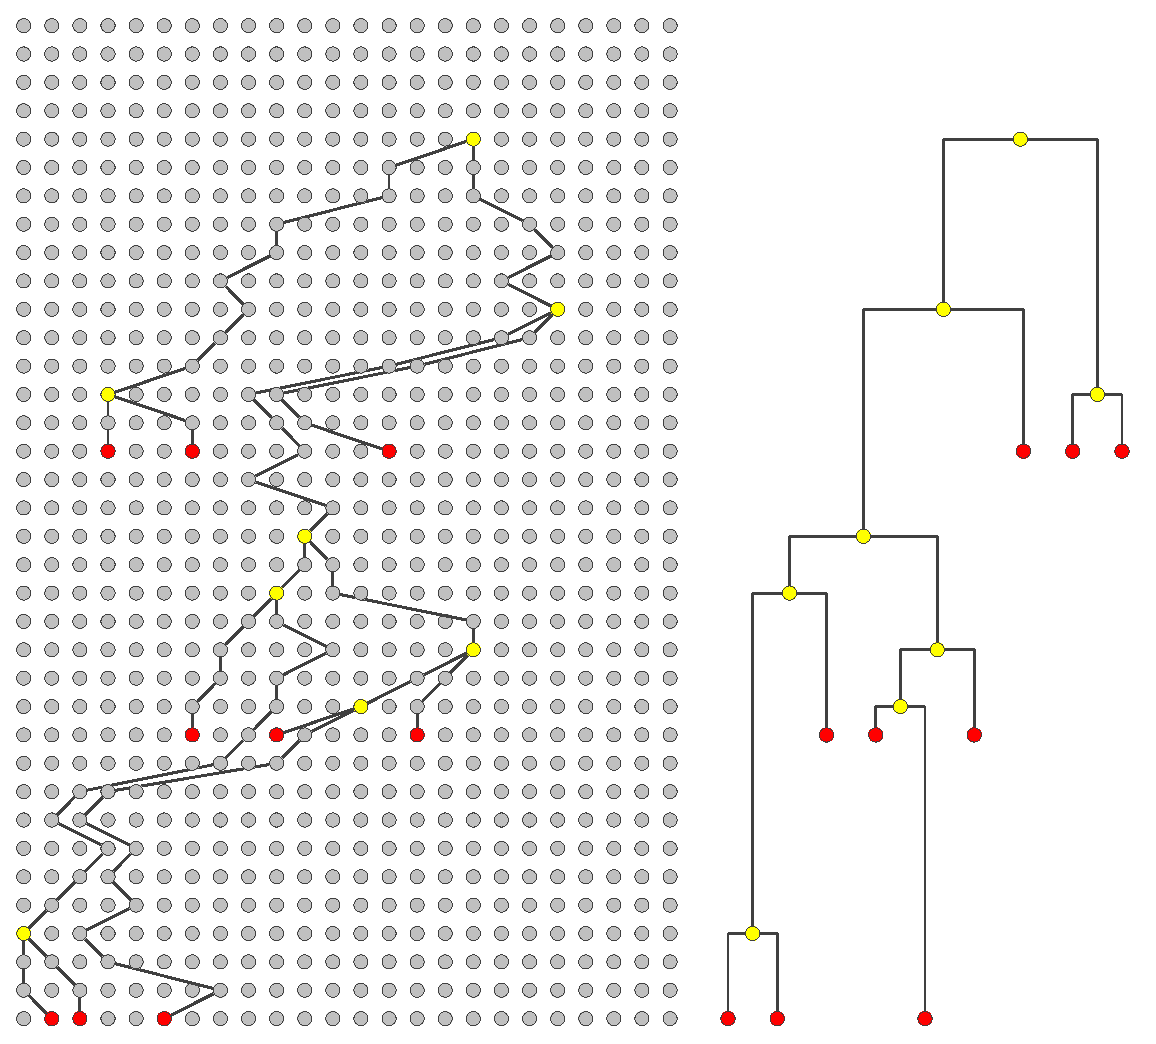
\includegraphics[width=\textwidth]{../images/serialConstant}%

\center{
Constant size}

\column{0.5\textwidth}

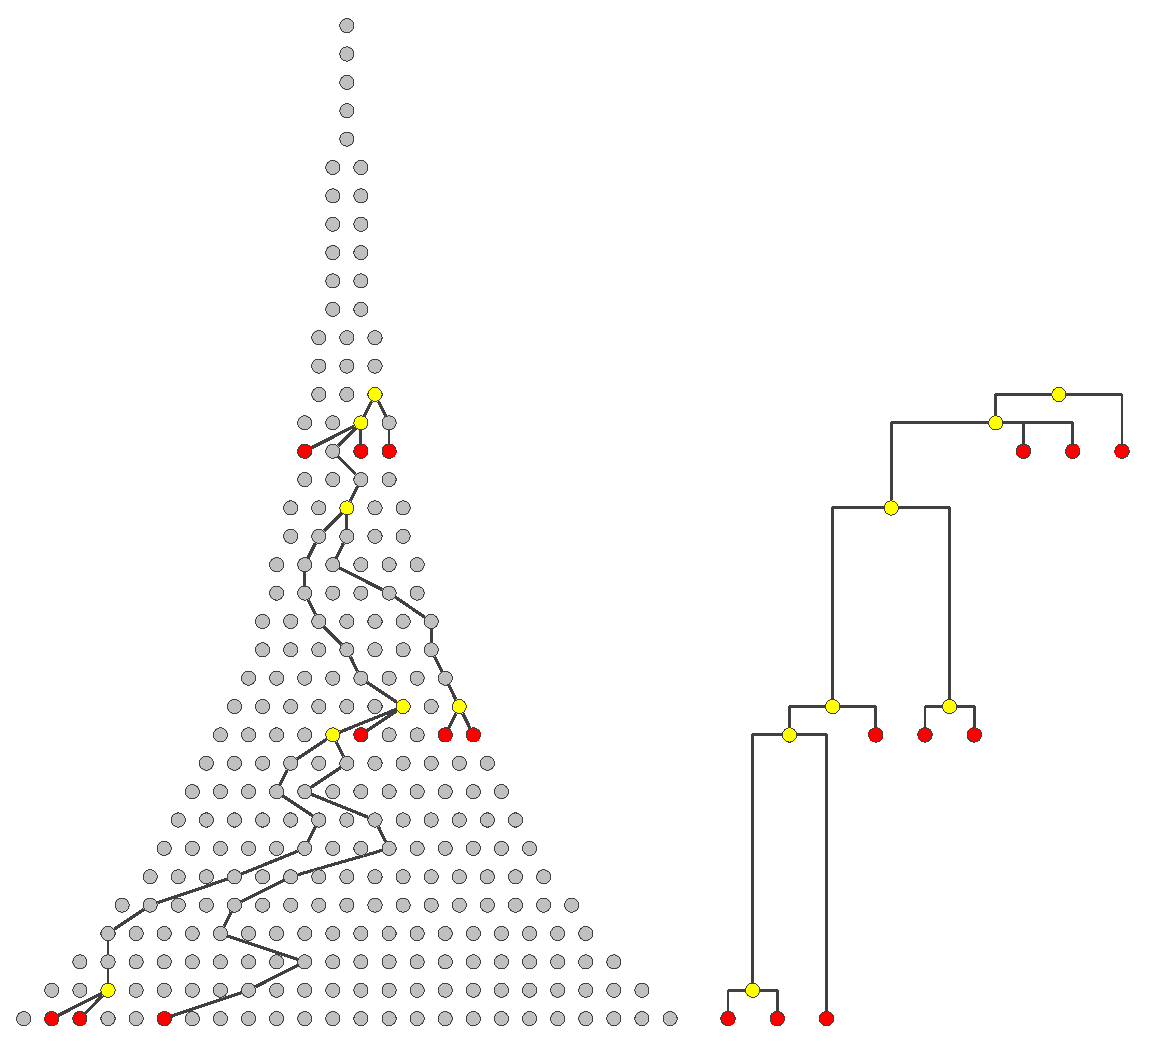
\includegraphics[width=\textwidth]{../images/serialExponential}%

\center{
Exponential growth}

\end{columns}

\end{frame}

\begin{frame}
\frametitle{Bayesian integration of uncertainty in genealogies}

\center{
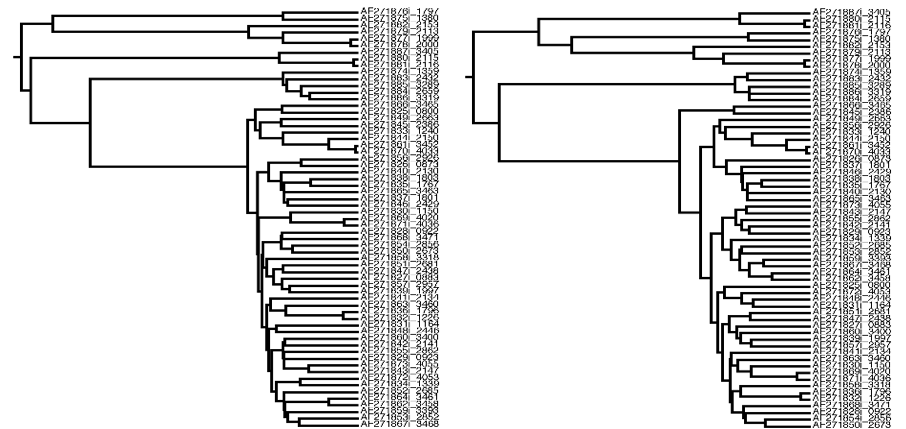
\includegraphics[scale=0.32]{../images/genealogicalUncertainty}
}

\smallskip

How similar are these two trees? Both of them are plausible given the data.
We can use Bayesian Markov-chain Monte Carlo to average the coalescent over all plausible trees.
\end{frame}
